\section{Lecture 2: \\ Quantum Protocols}
\SectionPage{}

\begin{frame}{Quantum Teleportation}

\bigskip

The IBM quantum computers currently do not support instructions after measurements, meaning we cannot run the quantum teleportation in its current form on real hardware. 

\bigskip

\begin{definition}[Principle of deferred measurement]
Measurements can always be moved from an intermediate stage of a quantum circuit to the end of the circuit.

If the measurement results are used at any stage of the circuit then the \alert{classically controlled operations} can be replaced by \alert{conditional quantum operations}.
\end{definition}

\end{frame}

\begin{frame}{Deferred Measurement}
 
 A consequence of the principle of deferred measurement is that \alert{measurement commutes with control}.
 
 \bigskip
 
\begin{center}
    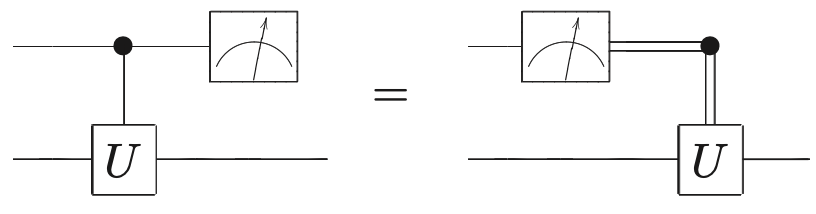
\includegraphics[width=0.85\textwidth]{img/DeferredMeasure.png}
\end{center}

\bigskip

\textbf{Exercise}

Prove the equality of the two circuits depicted above.


\end{frame}

\begin{frame}{Equivalent Teleportation Circuits}
 
\begin{center}
    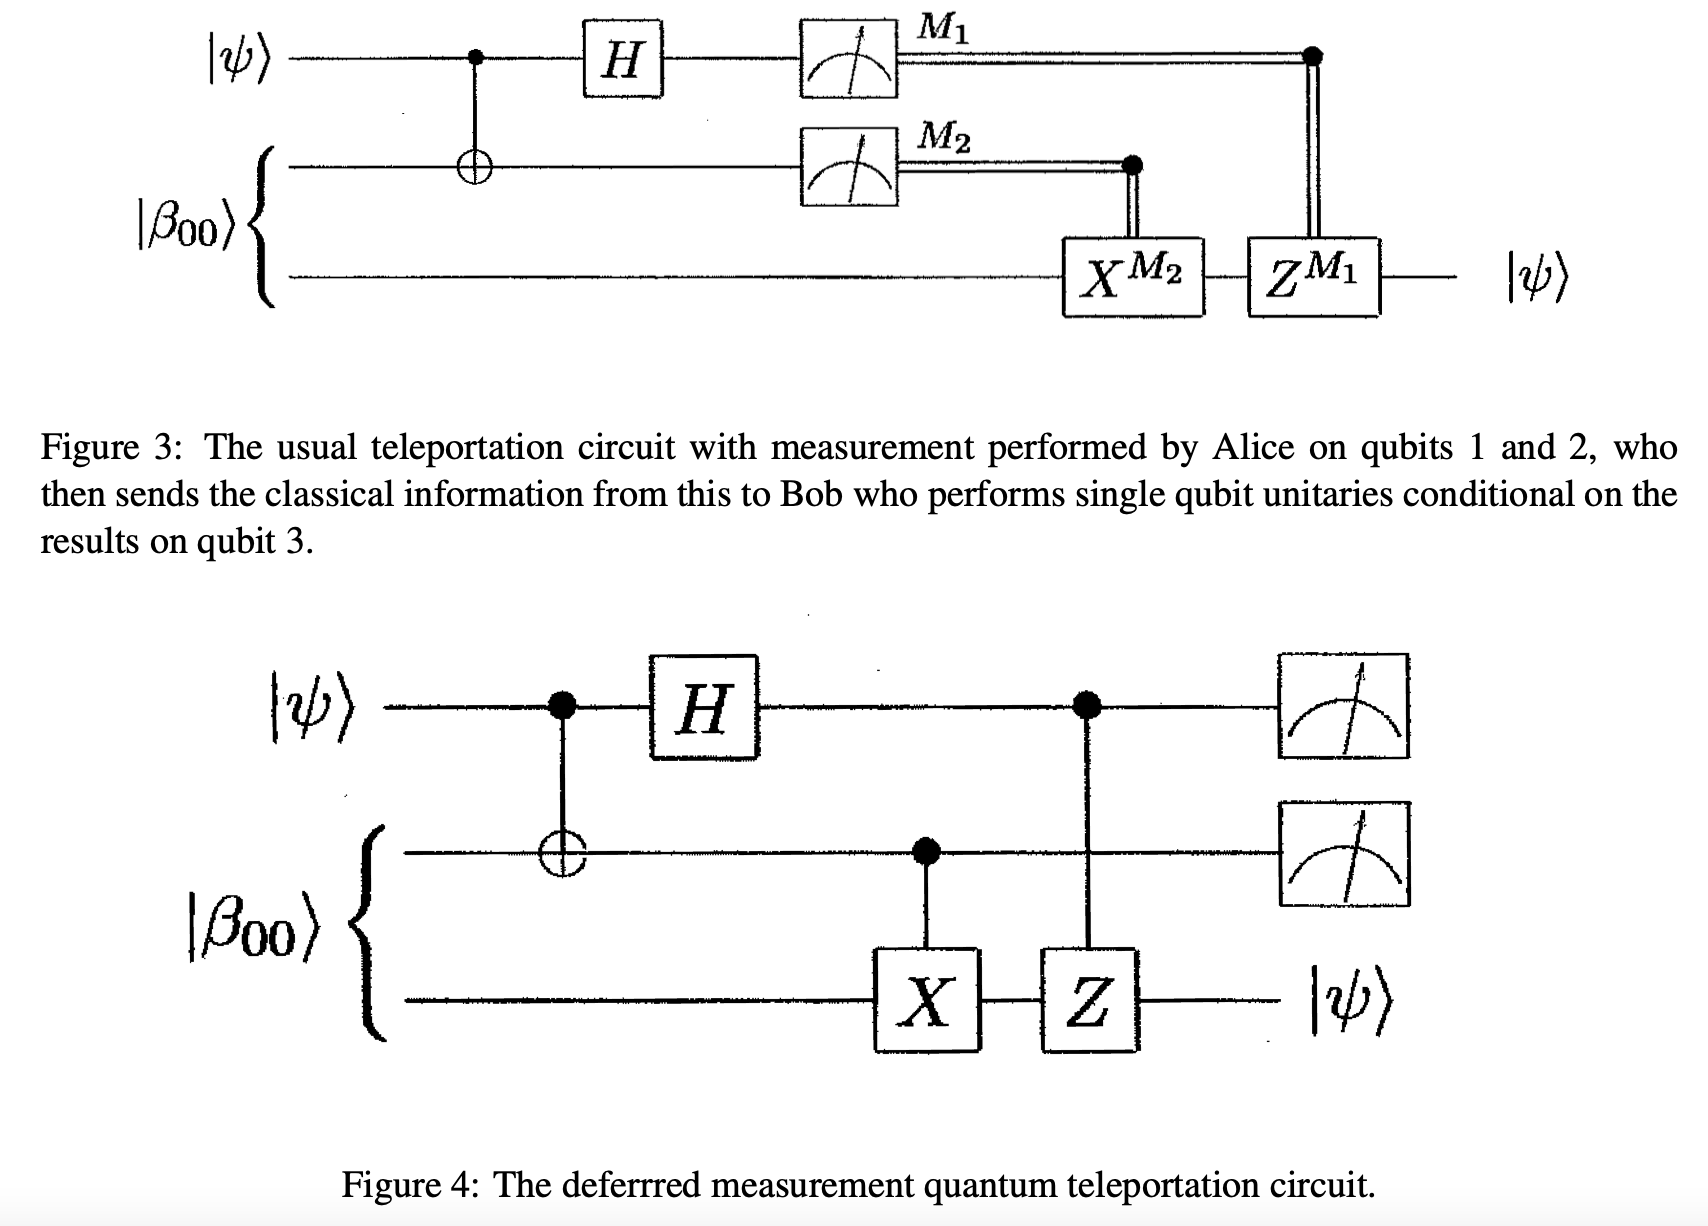
\includegraphics[width=0.80\textwidth]{img/EqivTelCircuits.png}
\end{center}
\end{frame}

\begin{frame}{Teleportation as State Transfer}
We are only interested in taking the input qubit $\psi$ to another location. We do not care what state we get in place of the original qubit at the sender. 

\begin{center}
    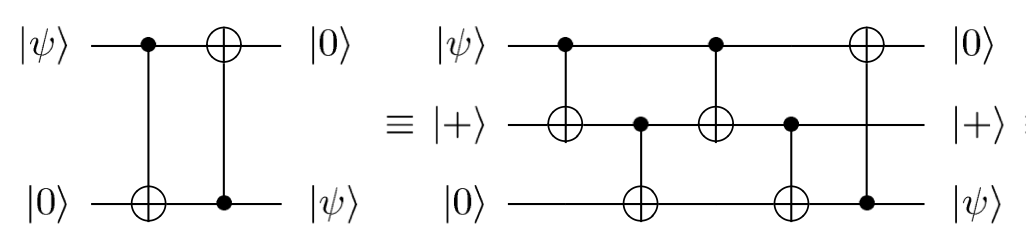
\includegraphics[width=0.80\textwidth]{img/state-transfer.png}
\end{center}

Other equivalent circuits:
\begin{center}
    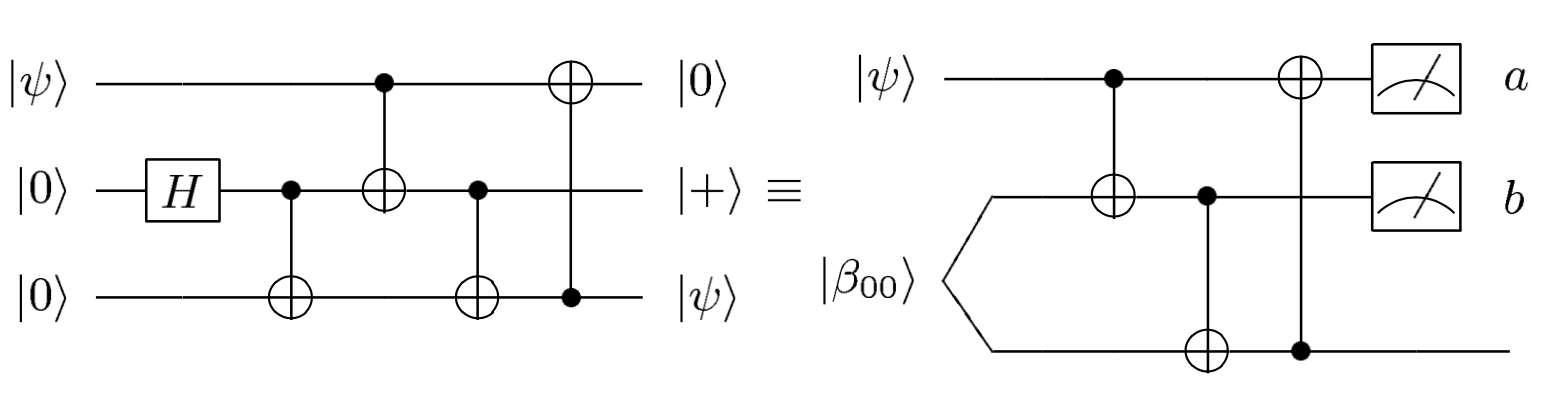
\includegraphics[width=0.80\textwidth]{img/Other-teleportation.png}
\end{center}
\end{frame}

\section{Exercise checking}
\SectionPage{}

% ============================================

\begin{frame}[fragile]{Exercise checking (1)}

\begin{itemize} 
\item Check your Qiskit installation
\end{itemize}

\begin{minted}{python}
import qiskit
qiskit.__qiskit_version__
\end{minted}

\bigskip No errors must appear (except the one regarding \code{matplotlib}, depending on the console you're using). 

\end{frame}

% ============================================

\begin{frame}[fragile]{Exercise checking (2)}

\begin{itemize} 
\item Define the circuits implementing the Bell states, simulate and execute them with any backend seen so far (including real machines)
\end{itemize}

\begin{minted}{python}
qc = QuantumCircuit(2, 2)
qc.h(0)
qc.cx(0, 1)

statevector_sim = Aer.get_backend('statevector_simulator')
statevector_result = execute(qc, backend=statevector_sim, shots=1)
    .result().get_statevector()

unitary_sim = Aer.get_backend('unitary_simulator')
unitary_result = execute(qc, backend=unitary_sim, shots=1)
    .result().get_unitary()
\end{minted}

\end{frame}


\begin{frame}[fragile]{Exercise checking (2)}

\begin{itemize} 
\item Define the circuits implementing the Bell states, simulate and execute them with any backend seen so far (including real machines)
\end{itemize}

\begin{minted}{python}
qc.measure([0, 1], [0, 1])
qasm_sim = Aer.get_backend('qasm_simulator')
qasm_result = execute(qc, backend=qasm_simulator, shots=1000)
    .result().get_statevector()

IBMQ.load_account()
santiago = IBMQ.get_provider().get_backend('ibmq_santiago')
counts = execute(qc, backend=santiago, shots=1000).result().get_counts()
\end{minted}

\end{frame}

% ============================================

\begin{frame}[fragile]{Exercise checking (3)}

\begin{itemize} 
\item How does the circuit size for arbitrary initialization grow when the number of qubit increases?
\end{itemize}

\begin{minted}{python}
from qiskit import * 
from qiskit.quantum_info.states.random import random_statevector

qubits = [1, 2, 3, 4, 5, 6, 7, 8]
sizes = []

for qubit in qubits:
	qc = QuantumCircuit(qubit)
	statevector = random_statevector(2**qubit)
	qc.initialize(statevector.data)
	qc2 = transpile(qc, basis_gates=['u3','cx'])
	sizes.append(qc2.size())
	
# sizes = [1, 6, 19, 48, 109, 234, 487, 996]
\end{minted}

\end{frame}


% ============================================

\begin{frame}[fragile]{Exercise checking (4)}

\begin{itemize} 
\item Try Deutsch-Jozsa
\end{itemize}

\bigskip See \url{qiskit.org/textbook/ch-algorithms/deutsch-jozsa.html}.

\end{frame}


\section{Quantum Teleportation}
\SectionPage{}

\begin{frame}{A note on Qiskit: which qubit is leftmost?}

\begin{center}
\begin{quantikz}[]
\lstick{\(\ket{\psi}\)}\qw
    & \gate[wires=3]{teleport}
    & \qw\rstick{\(\ket{b_1}\)} \\
\lstick{\(\ket{0}\)}\qw
    & \qw
    & \qw\rstick{\(\ket{b_2}\)} \\
\lstick{\(\ket{0}\)}\qw
    & \qw
    & \qw\rstick{\(\ket{\psi}\)}
\end{quantikz}
\end{center}

\bigskip At the beginning of the circuit the state is \( \ket{0} \otimes \ket{0} \otimes \ket{\psi} \)

\bigskip At the end of the circuit the state is \( \ket{\psi} \otimes \ket{b_2} \otimes \ket{b_1} \)

\end{frame}

% =====================================================

\begin{frame}[fragile]{The code (1)}

\begin{minted}[fontsize=\footnotesize]{python}
from qiskit.quantum_info.states.random import random_statevector
from qiskit import * \ import numpy as np

psi = random_statevector(2).data  
# array([0.75160912+0.04778984j, 0.49917654-0.42851213j])
qc = QuantumCircuit(3, 3)
qc.initialize(psi, 0)
sv_sim = Aer.get_backend('statevector_simulator')
statevector = execute(qc, sv_sim).result().get_statevector()
# array([0.75160912+0.04778984j, 0.49917654-0.42851213j,
#        0.        +0.j        , 0.        +0.j        ,
#        0.        +0.j        , 0.        +0.j        ,
#        0.        +0.j        , 0.        +0.j        ])
ket_zero = np.array([1, 0])
np.kron(np.kron(ket_zero, ket_zero), psi)
# array([0.75160912+0.04778984j, 0.49917654-0.42851213j,
#        0.        +0.j        , 0.        +0.j        ,
#        0.        +0.j        , 0.        +0.j        ,
#        0.        +0.j        , 0.        +0.j        ])
\end{minted}

\end{frame}


\begin{frame}{The protocol (1)}
\begin{quantikz}[]
\lstick[wires=2]{Alice}\qw
    & \gate{init(\ket{\psi})}
    & \qw \\
    \qw
    & \qw
    & \qw \\
\lstick{Bob}\qw
    & \qw
    & \qw
\end{quantikz}

\bigskip Alice own the qubit in state \(\ket{\psi} = \alpha \ket{0} + \beta \ket{1}\)
\end{frame}

% =========================================

\begin{frame}{The protocol (2)}
    
\begin{quantikz}[]
\lstick[wires=2]{Alice}\qw
    & \gate{init(\ket{\psi})}
    & \qw \\
    \qw
    & \gate[wires=2]{bell}
    & \qw\\
\lstick{\(\ket{0}\)}\qw
    & \qw
    & \qw
\end{quantikz}

\bigskip Alice and Bob shares a Bell state \(\frac{1}{\sqrt{2}} (\ket{00} + \ket{11})\)
\end{frame}

% =========================================

\begin{frame}[fragile]{Composed gates}

Hierarchical organization of the circuit

\begin{minted}{python}
def create_bell_circuit():
	bell_circuit = QuantumCircuit(2, name='bell')
	bell_circuit.h(0)
	bell_circuit.cx(0, 1)
	return bell_circuit

psi = random_statevector(2).data
qr = QuantumRegister(3, 'q')
crx = ClassicalRegister(1, 'crx')
crz = ClassicalRegister(1, 'crz')
qc = QuantumCircuit(qr, crx, crz)
qc.initialize(psi, qr[0])
qc.append(create_bell_circuit(), [qr[0], qr[1]])
\end{minted}
\end{frame}

% =========================================

\begin{frame}{The protocol (3)}
    
\begin{quantikz}[]
\lstick[wires=2]{Alice}\qw
    & \gate{init(\ket{\psi})}
    & \ctrl{1} 
    & \gate{H} 
    & \qw \\
    \qw
    & \gate[wires=2]{bell}
    & \targ{}
    & \qw
    & \qw\\
\lstick{\(\ket{0}\)}\qw
    & \qw
    & \qw
    & \qw
    & \qw
\end{quantikz}

\bigskip Alice applies CNOT and H, the state becomes
\begin{align*}
    \frac{1}{2} \Big( & \ket{00}(\alpha \ket{0} + \beta \ket{1}) \\
                    + & \ket{01}(\alpha \ket{1} + \beta \ket{0}) \\
                    + & \ket{10}(\alpha \ket{0} - \beta \ket{1}) \\
                    + & \ket{10}(\alpha \ket{1} - \beta \ket{0})\Big) 
\end{align*}
\end{frame}

% =========================================

\begin{frame}{The protocol (4)}
    
\begin{quantikz}[]
\lstick[wires=2]{Alice}\qw
    & \gate{init(\ket{\psi})}
    & \ctrl{1} 
    & \gate{H} 
    & \meter{}
    & \cw
    & \cwbend{2}\\
    \qw
    & \gate[wires=2]{bell}
    & \targ{}
    & \qw
    & \meter{}
    & \cwbend{1} \\
\lstick{\(\ket{0}\)}\qw
    & \qw
    & \qw
    & \qw
    & \qw
    & \gate{X}
    & \gate{Z}
    & \qw
\end{quantikz}

\bigskip Alice measures and send the two classical bits, Bob adjusts its qubit according to the received bits:
\begin{align*}
    00 & \to I \\
    01 & \to X \\
    10 & \to Z \\
    11 & \to ZX
\end{align*}
\end{frame}

% =========================================

\begin{frame}[fragile]{The code (2)}
\begin{minted}{python}
psi = random_statevector(2).data

qr = QuantumRegister(3, 'q')
crx = ClassicalRegister(1, 'crx')
crz = ClassicalRegister(1, 'crz')
qc = QuantumCircuit(qr, crx, crz)
qc.initialize(psi, qr[0])
qc.append(create_bell_circuit(), [qr[1], qr[2]])

qc.cx(qr[0], qr[1])
qc.h(qr[0])
qc.measure(qr[0], crz)
qc.measure(qr[1], crx)
qc.x(qr[2]).c_if(crx, 1)
qc.z(qr[2]).c_if(crz, 1)
\end{minted}
\end{frame}

\begin{frame}[fragile]{The code (3)}
\begin{minted}{python}
sv_sim = Aer.get_backend('statevector_simulator')
sv = execute(qc, sv_sim).result().get_statevector()
\end{minted}

\bigskip Is \code{sv} the state \( \ket{\psi} \otimes \ket{b_2} \otimes \ket{b_1} \)?
\end{frame}

% =========================================

\begin{frame}[fragile]{The code (4)}

What is we use deferred measurements? \bigskip

\begin{minted}{python}
qr = QuantumRegister(3, 'q')
crx = ClassicalRegister(1, 'crx')
crz = ClassicalRegister(1, 'crz')
qc = QuantumCircuit(qr, crx, crz)
qc.initialize(psi, qr[0])
qc.append(create_bell_circuit(), [qr[1], qr[2]])

qc.cx(qr[0], qr[1])
qc.h(qr[0])
qc.cx(qr[0], qr[2])
qc.cz(qr[1], qr[2])
qc.measure(qr[0], crz)
qc.measure(qr[1], crx)
\end{minted}
\end{frame}

% =========================================

\begin{frame}{Running on real quantum computers}

\begin{itemize}
    \item Deferred measurement is mandatory;
    \item How can I check if the state is exactly the one Alice wanted to send?
\end{itemize}
\end{frame}

\begin{frame}{Running on real quantum computers}

\begin{itemize}
    \item Deferred measurement is mandatory;
    \item How can I check if the state is exactly the one Alice wanted to send?
\end{itemize}

\bigskip
\begin{center}
\begin{quantikz}[]
\lstick{\(\ket{0}\)}\qw
    & \gate{init}
    & \gate[wires=3]{teleport}
    & \qw \\
\lstick{\(\ket{0}\)}\qw
    & \qw
    & \qw
    & \qw \\
\lstick{\(\ket{0}\)}\qw
    & \qw
    & \qw
    & \gate{init^{-1}}
    & \qw\rstick{\(\ket{0}\)}
\end{quantikz}
\end{center}

\qquad Check if the last qubit is zero

\end{frame}

% =========================================

\begin{frame}[fragile]{Inverse of \code{initialize} gate}

\begin{minted}{python}
from qiskit.extensions import Initialize
psi = random_statevector(2).data

init_gate = Initialize(psi)
init_gate.label = 'init'

inverse_init_gate = init_gate.gates_to_uncompute()

qc = QuantumCircuit(1)
qc.append(init_gate, [0])
qc.append(inverse_init_gate, [0])
sv = execute(qc, sv_sim).result().get_statevector()
# sv is ALMOST ket zero
\end{minted}

\end{frame}

% =========================================

\begin{frame}[fragile]{Inverse of \code{initialize} gate}

Be careful: \code{initialize} contains a non-linear \code{Reset} gate \bigskip

\begin{minted}{python}
init_gate = Initialize(psi)
init_gate.inverse() # error

inverse_init_gate = init_gate.gates_to_uncompute() # no reset
init_wo_reset = inverse_init_gate.inverse()

init_wo_reset.inverse() # ok
\end{minted}

\end{frame}

\begin{frame}{More on Quantum Teleportation}
Check this video of \emph{minutephysics}: \url{youtube.com/watch?v=dAaHHGHuy1c}
\end{frame}

\begin{frame}{Your turn!}
\begin{itemize}
    \item Demonstrate the equivalence of these circuits:
    \begin{center}
        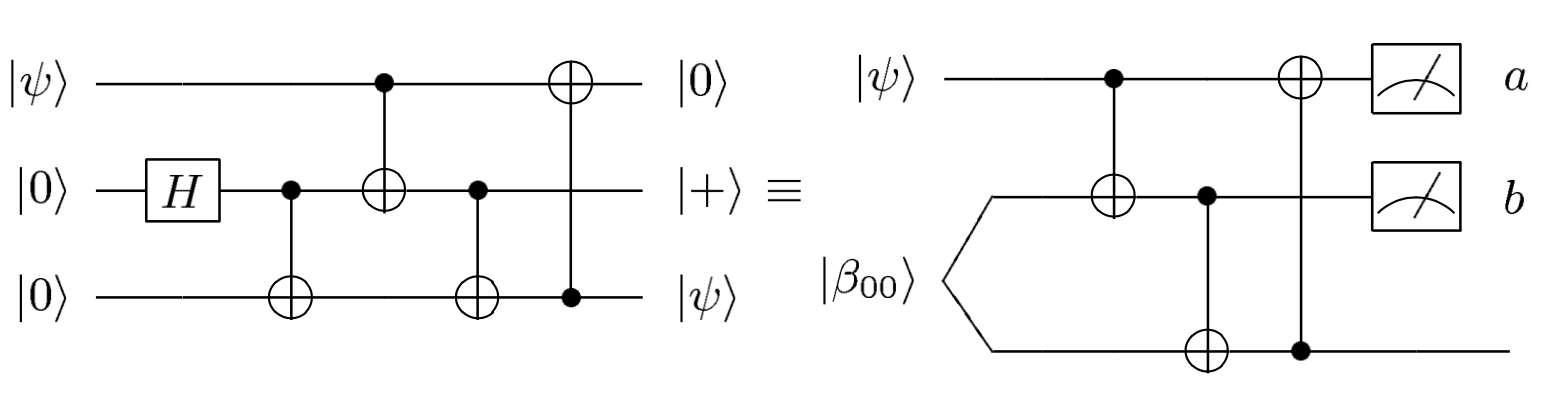
\includegraphics[width=0.80\textwidth]{img/Other-teleportation.png}
    \end{center}
    \item Run Quantum Teleportation
    \begin{itemize}
        \item \url{qiskit.org/textbook/ch-algorithms/teleportation.html}
        \item Explain how the network is used by Bob (Step 4) if the Bell state in input is $\frac{1}{\sqrt{2}}(\ket{01}+\ket{10})$.
    \end{itemize}
    \item Run Superdense Coding
    \begin{itemize}
        \item \url{qiskit.org/textbook/ch-algorithms/superdense-coding.html}
        \item Familiarize with the documentation!
    \end{itemize}
\end{itemize}

\end{frame}

% nota: eseguendo il circuito più volte il risultato dello statevector cambia, però facendo i conti sono i primi due qubit che cambiano e non il terzo
% controllare con metodo che fa 00psi, 01psi, 10psi, 11psi

